\documentclass[11pt]{article}
\usepackage{theme}
\usepackage{shortcuts}
% Document parameters
% Document title
\title{Assignment 1 (ML for TS) - MVA}
\author{
Soël Megdoud \email{Soel.Megdoud@ens-paris-saclay.fr} \\ % student 1
Julien Delavande \email{Julien.Delavande@ens-paris-saclay.fr} % student 2
}

\begin{document}
\maketitle

\section{Introduction}

\paragraph{Objective.} This assignment has three parts: questions about convolutional dictionary learning, spectral features, and a data study using the DTW. 

\paragraph{Warning and advice.} 
\begin{itemize}
    \item Use code from the tutorials as well as from other sources. Do not code yourself well-known procedures (e.g., cross-validation or k-means); use an existing implementation. 
    \item The associated notebook contains some hints and several helper functions.
    \item Be concise. Answers are not expected to be longer than a few sentences (omitting calculations).
\end{itemize}



\paragraph{Instructions.}
\begin{itemize}
    \item Fill in your names and emails at the top of the document.
    \item Hand in your report (one per pair of students) by Tuesday 28\textsuperscript{th} October 23:59 PM.
    \item Rename your report and notebook as follows:\\ \texttt{FirstnameLastname1\_FirstnameLastname2.pdf} and\\ \texttt{FirstnameLastname1\_FirstnameLastname2.ipynb}.\\
    For instance, \texttt{LaurentOudre\_CharlesTruong.pdf}.
    \item Upload your report (PDF file) and notebook (IPYNB file) using this link: \footnotesize{LINK}.
\end{itemize}


\section{Convolution dictionary learning}

\begin{exercise}
Consider the following Lasso regression:
\begin{equation}\label{eq:lasso}
    \min_{\beta\in\RR^p} \frac{1}{2}\norm{y-X\beta}^2_2 \quad + \quad \lambda \norm{\beta}_1
\end{equation}
where $y\in\RR^n$ is the response vector, $X\in\RR^{n\times p}$ the design matrix, $\beta\in\RR^p$ the vector of regressors and $\lambda>0$ the smoothing parameter.

Show that there exists $\lambda_{\max}$ such that the minimizer of~\eqref{eq:lasso} is $\mathbf{0}_p$ (a $p$-dimensional vector of zeros) for any $\lambda > \lambda_{\max}$. 
\end{exercise}

\begin{solution}  % QUESTION 1

    \begin{equation}
        \lambda{\max} = | X^T y |{\infty}
    \end{equation}
    
    Let’s consider the KKT conditions for the Lasso problem, which state that the gradient of the objective function with respect to $ \beta $ must be zero. This leads to the following system of equations:
    
    \[
    \frac{\partial f}{\partial \beta} = 0 \quad \text{which is equivalent to} \quad -X^T (y - X\beta) + \lambda , \text{sgn}(\beta) = \lambda , \text{sgn}(\beta) - X^T y + X^T X \beta = 0
    \]
    
    
    We will now assume $ \lambda > \lambda{\max} $, where:
    
    \[
    \lambda{\max} = | X^T y |{\infty}
    \]
    
    We will show by contradiction that $\beta = 0$ is the unique solution to the Lasso problem when $ \lambda > \lambda{\max} $. Suppose there exists an optimal solution $\beta \neq 0$.
    
    Since $\beta \neq 0$, there exists some index $i$ such that $ \beta_i \neq 0$. Without loss of generality, let’s assume $\beta_i > 0$ the case for $ \beta_i < 0$ is similar.
    
    We have:
    
    \[
    \lambda , \text{sgn}(\beta_i) - {X^T y}_i + {X^T X \beta}_i = \lambda - {X^T y}_i + (X^T X \beta)i
    \]
    
    Now, since we assumed $ \lambda > | X^T y |{\infty} $, we have $ \lambda > {X^T y}_i $. Therefore:
    
    \[
    \lambda - {X^T y}_i > 0
    \]
    
    Thus, the equation becomes:
    
    \[
    \lambda - {X^T y}_i + {X^T X \beta}_i > {X^T X \beta}_i > 0
    \]
    
    This implies that the KKT conditions are not satisfied for this non-zero \( \beta \) and that \( \beta = 0 \) is the unique solution for these \(\lambda\).
    
\end{solution}  % END QUESTION 1

\begin{exercise}
For a univariate signal $\mathbf{x}\in\mathbb{R}^n$ with $n$ samples, the convolutional dictionary learning task amounts to solving the following optimization problem:

\begin{equation}
\min_{(\mathbf{d}_k)_k, (\mathbf{z}_k)_k \\ \norm{\mathbf{d}_k}_2^2\leq 1} \quad\norm{\mathbf{x} - \sum_{k=1}^K \mathbf{z}_k * \mathbf{d}_k }^2_2 \quad + \quad\lambda \sum_{k=1}^K \norm{\mathbf{z}_k}_1
\end{equation}

where $\mathbf{d}_k\in\mathbb{R}^L$ are the $K$ dictionary atoms (patterns), $\mathbf{z}_k\in\mathbb{R}^{N-L+1}$ are activations signals, and $\lambda>0$ is the smoothing parameter.

Show that
\begin{itemize}
    \item for a fixed dictionary, the sparse coding problem is a lasso regression (explicit the response vector and the design matrix);
    \item for a fixed dictionary, there exists $\lambda_{\max}$ (which depends on the dictionary) such that the sparse codes are only 0 for any $\lambda > \lambda_{\max}$. 
\end{itemize}
\end{exercise}

\begin{solution}  % Question 2

Given the convolutional dictionary learning problem:

\[
\min_{(\mathbf{z}_k)_k} \|\mathbf{x} - \sum_{k=1}^K \mathbf{z}_k * \mathbf{d}_k\|_2^2 + \lambda \sum_{k=1}^K \|\mathbf{z}_k\|_1
\]

For a fixed dictionary, each convolution \(\mathbf{z}_k * \mathbf{d}_k\) is written as \(D_k \mathbf{z}_k\), where \(D_k \in \mathbb{R}^{n \times (n-L+1)}\) is a convolution matrix formed by sliding \(\mathbf{d}_k\). The objective becomes:

\[
\min_{\mathbf{z}} \|\mathbf{x} - D \mathbf{z}\|_2^2 + \lambda \|\mathbf{z}\|_1
\]

with \(D = [D_1, \dots, D_K]\), which is a Lasso regression. The threshold \(\lambda_{\max} = \|D^\top \mathbf{x}\|_\infty\) ensures that for \(\lambda > \lambda_{\max}\), the solution is \(\mathbf{z} = 0\).

\end{solution} % END QUESTION 2

\section{Spectral feature}

Let $X_n$ ($n=0,\dots, N-1)$ be a weakly stationary random process with zero mean and autocovariance function $\gamma(\tau):= \mathbb{E}(X_n X_{n+\tau})$.
Assume the autocovariances are absolutely summable, \ie $\sum_{\tau\in\mathbb{Z}} |\gamma(\tau)| < \infty$, and square summable, \ie $\sum_{\tau\in\mathbb{Z}} \gamma^2(\tau) < \infty$.
Denote the sampling frequency by $f_s$, meaning that the index $n$ corresponds to the time $n / f_s$. For simplicity, let $N$ be even.


The \textit{power spectrum} $S$ of the stationary random process $X$ is defined as the Fourier transform of the autocovariance function:
\begin{equation}
    S(f) := \sum_{\tau=-\infty}^{+\infty}\gamma(\tau)e^{-2\pi f\tau/f_s}.
\end{equation}
The power spectrum describes the distribution of power in the frequency space. 
Intuitively, large values of $S(f)$ indicate that the signal contains a sine wave at the frequency $f$.
There are many estimation procedures to determine this important quantity, which can then be used in a machine-learning pipeline.
In the following, we discuss the large sample properties of simple estimation procedures and the relationship between the power spectrum and the autocorrelation.

(Hint: use the many results on quadratic forms of Gaussian random variables to limit the number of calculations.)

\begin{exercise}
In this question, let $X_n$ ($n=0,\dots,N-1)$ be a Gaussian white noise.

\begin{itemize}
    \item Calculate the associated autocovariance function and power spectrum. (By analogy with the light, this process is called ``white'' because of the particular form of its power spectrum.)
\end{itemize}

\end{exercise}

\begin{solution} % QUESTION 3

For a Gaussian white noise process \(X_n\), we have:

\[
\mathbb{E}(X_n) = 0, \quad \text{and} \quad \mathbb{E}(X_n X_{n+\tau}) = \gamma(\tau) = \sigma^2 \delta(\tau),
\]
where \(\sigma^2\) is the variance of the process and \(\delta(\tau)\) is the Dirac delta function.

Thus, the autocovariance function is:
\[
\gamma(\tau) = \begin{cases} 
\sigma^2 & \text{if } \tau = 0, \\
0 & \text{otherwise}.
\end{cases}
\]

The power spectrum is the Fourier transform of the autocovariance function:
\[
S(f) = \sum_{\tau=-\infty}^{+\infty} \gamma(\tau) e^{-2\pi f \tau / f_s}.
\]

Since \(\gamma(\tau) = \sigma^2 \delta(\tau)\), this simplifies to:
\[
S(f) = \sigma^2 \sum_{\tau=-\infty}^{+\infty} \delta(\tau) e^{-2\pi f \tau / f_s} = \sigma^2.
\]

Thus, the power spectrum of white noise is constant across all frequencies, which is why it is called "white," analogous to white light containing all frequencies in equal measure.

\end{solution} % END QUESTION 3


\begin{exercise}
A natural estimator for the autocorrelation function is the sample autocovariance
\begin{equation}
    \hat{\gamma}(\tau) := (1/N) \sum_{n=0}^{N-\tau-1} X_n X_{n+\tau}
\end{equation}
for $\tau=0,1,\dots,N-1$ and $\hat{\gamma}(\tau):=\hat{\gamma}(-\tau)$ for $\tau=-(N-1),\dots,-1$.
\begin{itemize}
    \item Show that $\hat{\gamma}(\tau)$ is a biased estimator of $\gamma(\tau)$ but asymptotically unbiased.
    What would be a simple way to de-bias this estimator?
\end{itemize}

\end{exercise}

\begin{solution} % QUESTION 4

The sample autocovariance is defined as:

\[
\hat{\gamma}(\tau) = \frac{1}{N} \sum_{n=0}^{N-\tau-1} X_n X_{n+\tau}, \quad \tau = 0, 1, \dots, N-1.
\]

We want to show that \(\hat{\gamma}(\tau)\) is biased but asymptotically unbiased. The true autocovariance is:

\[
\gamma(\tau) = \mathbb{E}(X_n X_{n+\tau}).
\]

Now, consider the expectation of the sample autocovariance:

\[
\mathbb{E}[\hat{\gamma}(\tau)] = \frac{1}{N} \sum_{n=0}^{N-\tau-1} \mathbb{E}(X_n X_{n+\tau}) = \frac{N-\tau}{N} \gamma(\tau).
\]

Thus, we have:

\[
\mathbb{E}[\hat{\gamma}(\tau)] = \left(1 - \frac{\tau}{N}\right) \gamma(\tau).
\]

This shows that \(\hat{\gamma}(\tau)\) is a biased estimator because \(\mathbb{E}[\hat{\gamma}(\tau)] \neq \gamma(\tau)\). However, as \(N \to \infty\), the bias term \(\frac{\tau}{N} \to 0\), making \(\hat{\gamma}(\tau)\) \textbf{asymptotically unbiased}.

A simple way to de-bias this estimator is to scale \(\hat{\gamma}(\tau)\) by \(\frac{N}{N-\tau}\), yielding the corrected estimator:

\[
\hat{\gamma}_{\text{debias}}(\tau) = \frac{N}{N-\tau} \hat{\gamma}(\tau).
\]

\end{solution} % END QUESTION 4

\begin{exercise}
Define the discrete Fourier transform of the random process $\{X_n\}_n$ by
\begin{equation}
    J(f) := (1/\sqrt{N})\sum_{n=0}^{N-1} X_n e^{-2\pi\iu f n/f_s}
\end{equation}
The \textit{periodogram} is the collection of values $|J(f_0)|^2$, $|J(f_1)|^2$, \dots, $|J(f_{N/2})|^2$ where $f_k = f_s k/N$.
(They can be efficiently computed using the Fast Fourier Transform.)
\begin{itemize}
    \item Write $|J(f_k)|^2$ as a function of the sample autocovariances.
    \item For a frequency $f$, define $f^{(N)}$ the closest Fourier frequency $f_k$ to $f$.
    Show that $|J(f^{(N)})|^2$ is an asymptotically unbiased estimator of $S(f)$ for $f>0$.
\end{itemize}
\end{exercise}

\begin{solution} % QUESTION 5

\begin{itemize}
    

\item Step 1: Periodogram as a Function of Autocovariances

The discrete Fourier transform (DFT) of the process \(\{X_n\}_n\) is given by:

\[
J(f) = \frac{1}{\sqrt{N}} \sum_{n=0}^{N-1} X_n e^{-2\pi i f n / f_s}.
\]

The periodogram is the collection of values \(|J(f_k)|^2\) for \(k = 0, 1, \dots, N/2\), where \(f_k = f_s k / N\). Using the inverse Fourier transform, we can express \(|J(f_k)|^2\) as a function of the sample autocovariances:

\[
|J(f_k)|^2 = \frac{1}{N} \sum_{\tau=-N+1}^{N-1} \hat{\gamma}(\tau) e^{-2\pi i f_k \tau / f_s}.
\]

This shows that the periodogram is essentially the discrete Fourier transform of the sample autocovariances.

\item Step 2: Asymptotic Unbiasedness of the Periodogram

Let \(f^{(N)}\) denote the Fourier frequency closest to \(f\). We want to show that \(|J(f^{(N)})|^2\) is an asymptotically unbiased estimator of the true power spectrum \(S(f)\).

Since \(\hat{\gamma}(\tau)\) is asymptotically unbiased for \(\gamma(\tau)\), and the periodogram is the Fourier transform of \(\hat{\gamma}(\tau)\), it follows that the periodogram \(|J(f^{(N)})|^2\) is an asymptotically unbiased estimator of \(S(f)\) for \(f > 0\).

For large \(N\), we have:

\[
\mathbb{E}[|J(f^{(N)})|^2] \to S(f),
\]

which proves the asymptotic unbiasedness of the periodogram as an estimator of the power spectrum \(S(f)\).
\end{itemize}

    
\end{solution} % END QUESTION 5

\begin{exercise}\label{ex:wn-exp}
    In this question, let $X_n$ ($n=0,\dots,N-1)$ be a Gaussian white noise with variance $\sigma^2=1$ and set the sampling frequency to $f_s=1$ Hz
    \begin{itemize}
        \item For $N\in\{200, 500, 1000\}$, compute the \textit{sample autocovariances} ($\hat{\gamma}(\tau)$ vs $\tau$) for 100 simulations of $X$.
        Plot the average value as well as the average $\pm$, the standard deviation.
        What do you observe?
        \item For $N\in\{200, 500, 1000\}$, compute the \textit{periodogram} ($|J(f_k)|^2$ vs $f_k$) for 100 simulations of $X$.
        Plot the average value as well as the average $\pm$, the standard deviation.
        What do you observe?
    \end{itemize}
    Add your plots to Figure~\ref{fig:wn-exp}.
    
\begin{figure}
    \centering
    \begin{minipage}[t]{0.3\textwidth}
    \centerline{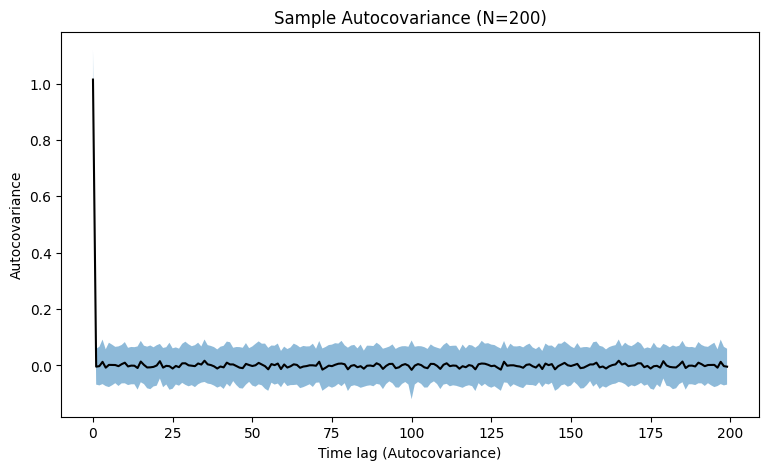
\includegraphics[width=\textwidth]{figures/autocovariance_N200.png}}
    \centerline{Autocovariance ($N=200$)}
    \end{minipage}
    \begin{minipage}[t]{0.3\textwidth}
    \centerline{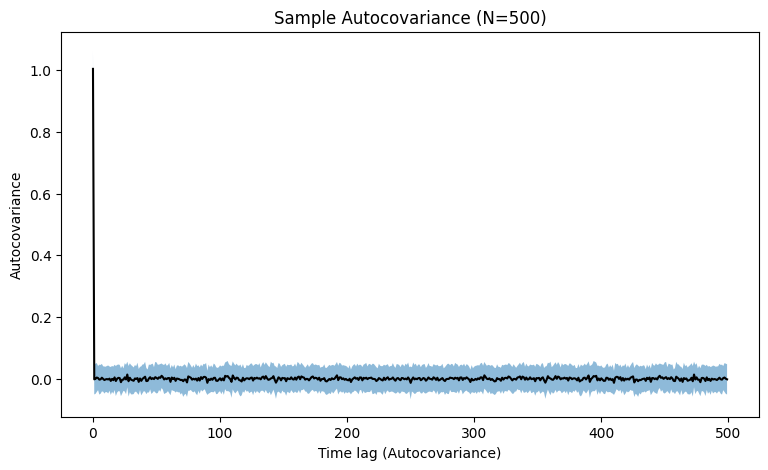
\includegraphics[width=\textwidth]{figures/autocovariance_N500.png}}
    \centerline{Autocovariance ($N=500$)}
    \end{minipage}
    \begin{minipage}[t]{0.3\textwidth}
    \centerline{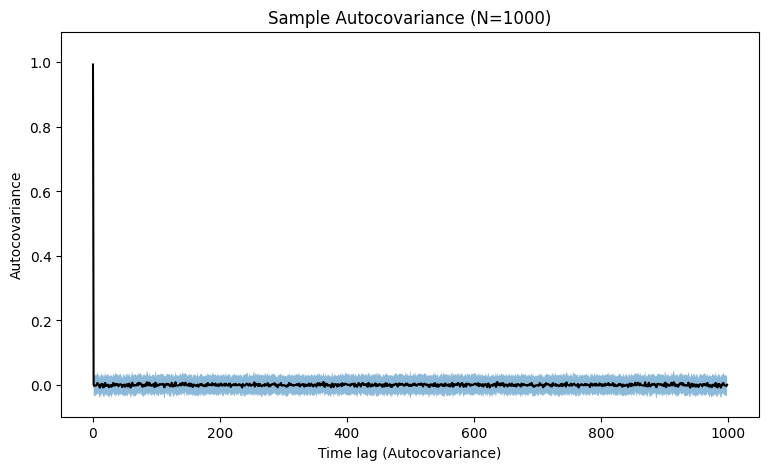
\includegraphics[width=\textwidth]{figures/autocovariance_N1000.png}}
    \centerline{Autocovariance ($N=1000$)}
    \end{minipage}
    \vskip1em
    \begin{minipage}[t]{0.3\textwidth}
    \centerline{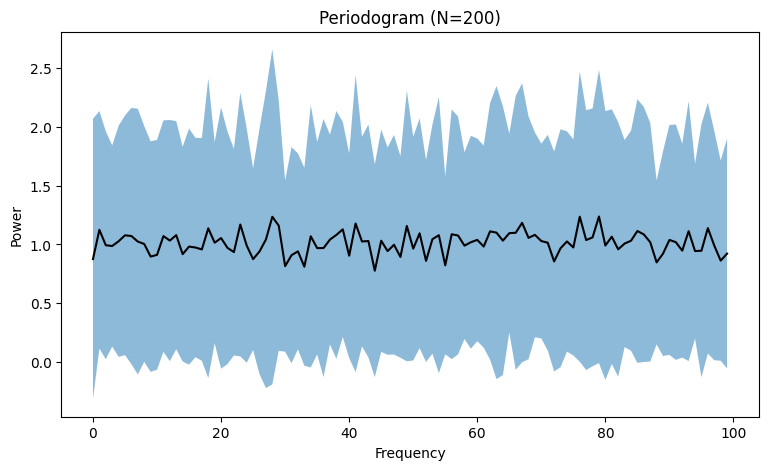
\includegraphics[width=\textwidth]{figures/periodogram_N200.png}}
    \centerline{Periodogram ($N=200$)}
    \end{minipage}
    \begin{minipage}[t]{0.3\textwidth}
    \centerline{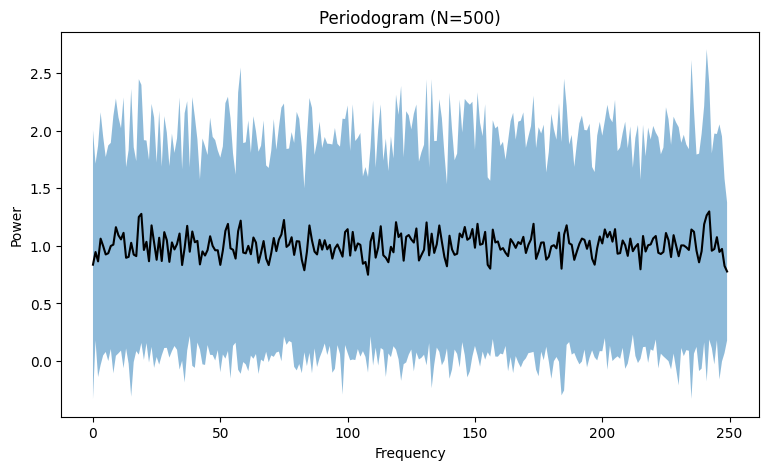
\includegraphics[width=\textwidth]{figures/periodogram_N500.png}}
    \centerline{Periodogram ($N=500$)}
    \end{minipage}
    \begin{minipage}[t]{0.3\textwidth}
    \centerline{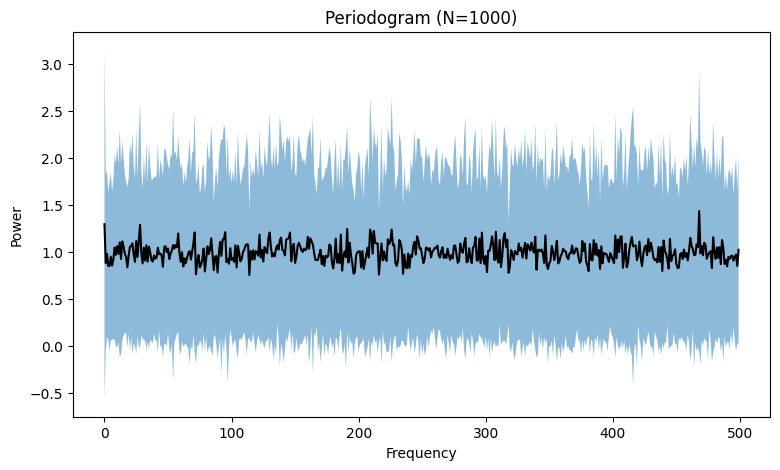
\includegraphics[width=\textwidth]{figures/periodogram_N1000.png}}
    \centerline{Periodogram ($N=1000$)}
    \end{minipage}
    \vskip1em
    \caption{Autocovariances and periodograms of a Gaussian white noise (see Question~\ref{ex:wn-exp}).}
    \label{fig:wn-exp}
\end{figure}

\end{exercise}

\begin{solution} % QUESTION 6

    For both the sample autocovariances and periodograms, here are the key observations from the plots:
    
    \paragraph{Sample Autocovariances:}
    \begin{itemize}    
        \item For each value of $N$ (200, 500, 1000), the sample autocovariances have a sharp peak at $\tau = 0$, which is consistent with the fact that Gaussian white noise is uncorrelated. 
        \item As $N$ increases, the variance of the sample autocovariances decreases, which leads to a tighter confidence interval around the mean. This suggests that the estimate of the autocovariance becomes more reliable as the number of samples grows.
        \item The values of the autocovariances at lags $\tau \neq 0$ are close to zero, which aligns with the theoretical property of white noise being uncorrelated across time.
    \end{itemize}

    \paragraph{Periodograms:}
    \begin{itemize} 
        \item The periodograms show that for all values of $N$, the power is roughly constant across frequencies, which matches the expected flat power spectral density of Gaussian white noise.
        \item As $N$ increases, the standard deviation of the periodogram decreases, meaning that the estimate of the power at each frequency becomes more stable with more data.
        \item Even though the periodogram is asymptotically unbiased, the variability (especially for smaller $N$) is quite high, which is reflected in the large fluctuations observed in the plots. This demonstrates the erratic behavior of the periodogram for small sample sizes.
    \end{itemize}

    In summary, both the sample autocovariance and periodogram plots become more reliable and less variable as $N$ increases, which confirms the consistency of these estimators for large $N$.
    
\end{solution} % END QUESTION 6
    

\begin{exercise}
    We want to show that the estimator $\hat{\gamma}(\tau)$ is consistent, \ie it converges in probability when the number $N$ of samples grows to $\infty$ to the true value ${\gamma}(\tau)$.
    In this question, assume that $X$ is a wide-sense stationary \textit{Gaussian} process.
    \begin{itemize}
        \item Show that for $\tau>0$ 
    \begin{equation}
       \text{var}(\hat{\gamma}(\tau)) = (1/N) \sum_{n=-(N-\tau-1)}^{n=N-\tau-1} \left(1 - \frac{\tau + |n|}{N}\right) \left[\gamma^2(n) + \gamma(n-\tau)\gamma(n+\tau)\right].
    \end{equation}
    (Hint: if $\{Y_1, Y_2, Y_3, Y_4\}$ are four centered jointly Gaussian variables, then $\mathbb{E}[Y_1 Y_2 Y_3 Y_4] = \mathbb{E}[Y_1 Y_2]\mathbb{E}[Y_3 Y_4] + \mathbb{E}[Y_1 Y_3]\mathbb{E}[Y_2 Y_4] + \mathbb{E}[Y_1 Y_4]\mathbb{E}[Y_2 Y_3]$.) 
    \item Conclude that $\hat{\gamma}(\tau)$ is consistent.
    \end{itemize}
\end{exercise}

\begin{solution} % QUESTION 7
    \begin{itemize}
        \item \begin{proof}
    Let $X = \{X_n\}$ be a wide-sense stationary Gaussian process with zero mean, i.e., $\mathbb{E}[X_n] = 0$ for all $n$. The empirical estimator of the autocovariance at lag $\tau > 0$ is:
    \[
    \hat{\gamma}(\tau) = \frac{1}{N} \sum_{n=0}^{N-\tau-1} X_n X_{n+\tau}.
    \]
    
    First, note that:
    \[
    \mathbb{E}[\hat{\gamma}(\tau)] = \gamma(\tau),
    \]
    since $\mathbb{E}[X_n X_{n+\tau}] = \gamma(\tau)$ due to stationarity.
    
    To compute the variance $\text{var}(\hat{\gamma}(\tau))$, we have:
    \[
    \text{var}(\hat{\gamma}(\tau)) = \mathbb{E}[\hat{\gamma}^2(\tau)] - \gamma^2(\tau),
    \]
    where
    \[
    \mathbb{E}[\hat{\gamma}^2(\tau)] = \frac{1}{N^2} \sum_{n=0}^{N-\tau-1} \sum_{m=0}^{N-\tau-1} \mathbb{E}[X_n X_{n+\tau} X_m X_{m+\tau}].
    \]
    
    Using the hint for jointly Gaussian zero-mean variables, we get:
    
    \[
    \mathbb{E}[X_n X_{n+\tau} X_m X_{m+\tau}] = \gamma^2(\tau) + \gamma^2(n - m) + \gamma(n - m - \tau) \gamma(n - m + \tau).
    \]
    
    Thus,
    \[
    \mathbb{E}[\hat{\gamma}^2(\tau)] = \frac{1}{N^2} \sum_{n=0}^{N-\tau-1} \sum_{m=0}^{N-\tau-1} \left[ \gamma^2(\tau) + \gamma^2(n - m) + \gamma(n - m - \tau)\gamma(n - m + \tau) \right].
    \]
    
    Let $k = n - m$. The number of pairs $(n, m)$ such that $n - m = k$ is $(N - \tau - |k|)$ for $|k| \leq N - \tau - 1$. Therefore,
    \[
    \mathbb{E}[\hat{\gamma}^2(\tau)] = \frac{1}{N^2} \sum_{k=-(N-\tau-1)}^{N-\tau-1} (N - \tau - |k|) \left[ \gamma^2(\tau) + \gamma^2(k) + \gamma(k - \tau)\gamma(k + \tau) \right].
    \]
    
    Subtracting $\gamma^2(\tau)$, we obtain:
    \[
    \text{var}(\hat{\gamma}(\tau)) = \frac{1}{N^2} \sum_{k=-(N-\tau-1)}^{N-\tau-1} (N - \tau - |k|) \left[ \gamma^2(k) + \gamma(k - \tau)\gamma(k + \tau) \right].
    \]
    
    Rewriting, we get:
    \[
    \text{var}(\hat{\gamma}(\tau)) = \frac{1}{N} \sum_{k=-(N-\tau-1)}^{N-\tau-1} \left(1 - \frac{\tau + |k|}{N}\right) \left[ \gamma^2(k) + \gamma(k - \tau)\gamma(k + \tau) \right].
    \]
    
    \end{proof}
    
        \item Since $\gamma(k)$ is bounded and the term $\frac{\tau + |k|}{N} \to 0$ as $N \to \infty$, we have:
    \[
    \lim_{N \to \infty} \text{var}(\hat{\gamma}(\tau)) = 0.
    \]
    
    Therefore, $\hat{\gamma}(\tau)$ converges in probability to $\gamma(\tau)$, and thus it is a consistent estimator.
    \end{itemize}
        
\end{solution}  % END QUESTION 7
    
Contrary to the correlogram, the periodogram is not consistent.
It is one of the most well-known estimators that is asymptotically unbiased but not consistent.
In the following question, this is proven for Gaussian white noise, but this holds for more general stationary processes.
\begin{exercise}
    Assume that $X$ is a Gaussian white noise (variance $\sigma^2$) and let $A(f):=\sum_{n=0}^{N-1} X_n \cos(-2\pi f n/f_s$ and $B(f):=\sum_{n=0}^{N-1} X_n \sin(-2\pi f n/f_s$.
    Observe that $J(f) = (1/N) (A(f) + \iu B(f))$.
    \begin{itemize}
        \item Derive the mean and variance of $A(f)$ and $B(f)$ for $f=f_0, f_1,\dots, f_{N/2}$ where $f_k=f_s k/N$.
        \item What is the distribution of the periodogram values $|J(f_0)|^2$, $|J(f_1)|^2$, \dots, $|J(f_{N/2})|^2$.
        \item What is the variance of the $|J(f_k)|^2$? Conclude that the periodogram is not consistent.
        \item Explain the erratic behavior of the periodogram in Question~\ref{ex:wn-exp} by looking at the covariance between the $|J(f_k)|^2$.
    \end{itemize}
    
\end{exercise}

\begin{solution}
    \begin{proof}
    \textbf{(a) Mean and Variance of \(A(f_k)\) and \(B(f_k)\):}
    
    Given \(X_n\) are independent Gaussian random variables with mean zero and variance \(\sigma^2\), we have:
    \[
    A(f_k) = \sum_{n=0}^{N-1} X_n \cos\left(-2\pi f_k n / f_s\right),
    \]
    \[
    B(f_k) = \sum_{n=0}^{N-1} X_n \sin\left(-2\pi f_k n / f_s\right),
    \]
    where \(f_k = \frac{f_s k}{N}\), for \(k = 0, 1, \dots, N/2\).
    
    \emph{Mean}:
    \[
    \mathbb{E}[A(f_k)] = \sum_{n=0}^{N-1} \mathbb{E}[X_n] \cos\left(-2\pi f_k n / f_s\right) = 0,
    \]
    \[
    \mathbb{E}[B(f_k)] = \sum_{n=0}^{N-1} \mathbb{E}[X_n] \sin\left(-2\pi f_k n / f_s\right) = 0.
    \]
    
    \emph{Variance}:
    \begin{align*}
    \text{Var}[A(f_k)] &= \mathbb{E}[A(f_k)^2] = \sum_{n=0}^{N-1} \mathbb{E}[X_n^2] \cos^2\left(2\pi k n / N\right) \\
    &= \sigma^2 \sum_{n=0}^{N-1} \cos^2\left(2\pi k n / N\right) = \frac{\sigma^2 N}{2},
    \end{align*}
    since \(\sum_{n=0}^{N-1} \cos^2\left(2\pi k n / N\right) = N/2\).
    
    Similarly,
    \[
    \text{Var}[B(f_k)] = \frac{\sigma^2 N}{2}.
    \]
    
    \textbf{(b) Distribution of \(|J(f_k)|^2\):}
    
    Since \(A(f_k)\) and \(B(f_k)\) are linear combinations of independent Gaussian variables, they are jointly Gaussian. The covariance between \(A(f_k)\) and \(B(f_k)\) is:
    \begin{align*}
    \text{Cov}[A(f_k), B(f_k)] &= \mathbb{E}[A(f_k) B(f_k)] \\
    &= \sum_{n=0}^{N-1} \mathbb{E}[X_n^2] \cos\left(2\pi k n / N\right) \sin\left(2\pi k n / N\right) \\
    &= \sigma^2 \sum_{n=0}^{N-1} \frac{\sin\left(4\pi k n / N\right)}{2} = 0,
    \end{align*}
    since the sum of \(\sin\left(4\pi k n / N\right)\) over one or multiple periods is zero.
    
    Thus, \(A(f_k)\) and \(B(f_k)\) are independent Gaussian random variables with mean zero and variance \(\sigma^2 N/2\).
    
    The periodogram at frequency \(f_k\) is:
    \[
    |J(f_k)|^2 = \left|\frac{A(f_k) + i B(f_k)}{N}\right|^2 = \frac{A(f_k)^2 + B(f_k)^2}{N^2}.
    \]
    
    Define \(Z = \frac{\sqrt{2}}{\sigma \sqrt{N}} (A(f_k) + i B(f_k))\), then \(Z\) is a complex Gaussian random variable with independent standard normal real and imaginary parts. Therefore,
    \[
    |Z|^2 = \left(\frac{\sqrt{2}}{\sigma \sqrt{N}}\right)^2 (A(f_k)^2 + B(f_k)^2) = \frac{2}{\sigma^2 N} (A(f_k)^2 + B(f_k)^2) \sim \chi^2_2,
    \]
    where \(\chi^2_2\) denotes the chi-squared distribution with 2 degrees of freedom.
    
    Thus,
    \[
    |J(f_k)|^2 = \frac{\sigma^2}{N} \cdot \frac{|Z|^2}{2} \sim \frac{\sigma^2}{N} \cdot \text{Exp}(1),
    \]
    since \(\chi^2_2/2\) follows an exponential distribution with mean 1.
    
    \textbf{(c) Variance of \(|J(f_k)|^2\) and Non-Consistency:}
    
    The mean and variance of \(|J(f_k)|^2\) are:
    \[
    \mathbb{E}[|J(f_k)|^2] = \frac{\sigma^2}{N},
    \]
    \[
    \text{Var}[|J(f_k)|^2] = \left(\frac{\sigma^2}{N}\right)^2 \text{Var}\left[\frac{\chi^2_2}{2}\right] = \left(\frac{\sigma^2}{N}\right)^2.
    \]
    
    The variance does not tend to zero relative to the mean as \(N \to \infty\):
    \[
    \frac{\text{Var}[|J(f_k)|^2]}{\left(\mathbb{E}[|J(f_k)|^2]\right)^2} = 1.
    \]
    
    Since the variance of \(|J(f_k)|^2\) does not vanish as \(N\) increases, the periodogram \(|J(f_k)|^2\) is not consistent.
    
    \textbf{(d) Covariance Between \(|J(f_k)|^2\) and \(|J(f_l)|^2\):}
    
    The covariance between \(|J(f_k)|^2\) and \(|J(f_l)|^2\) for \(k \ne l\) is non-zero due to the overlapping sums in \(A(f_k)\) and \(A(f_l)\), and similarly for \(B(f_k)\) and \(B(f_l)\). This leads to:
    \[
    \text{Cov}[|J(f_k)|^2, |J(f_l)|^2] = \frac{\sigma^4}{N^2} \left| \sum_{n=0}^{N-1} e^{-2\pi i (f_k - f_l) n / f_s} \right|^2.
    \]
    
    This covariance does not vanish as \(N \to \infty\), causing the periodogram values at different frequencies to be correlated. This correlation leads to the erratic behavior observed in the periodogram, as fluctuations at one frequency affect those at others, preventing the periodogram from converging smoothly as \(N\) increases.
    \end{proof}
        
    \end{solution}
    

\begin{exercise}\label{q:barlett}
    As seen in the previous question, the problem with the periodogram is the fact that its variance does not decrease with the sample size.
    A simple procedure to obtain a consistent estimate is to divide the signal into $K$ sections of equal durations, compute a periodogram on each section, and average them.
    Provided the sections are independent, this has the effect of dividing the variance by $K$. 
    This procedure is known as Bartlett's procedure.
    \begin{itemize}
        \item Rerun the experiment of Question~\ref{ex:wn-exp}, but replace the periodogram by Barlett's estimate (set $K=5$). What do you observe?
    \end{itemize}
    Add your plots to Figure~\ref{fig:barlett}.
\end{exercise}

\begin{solution}


    When applying Bartlett's procedure, we divide the signal into \( K = 5 \) equal sections, compute the periodogram for each section, and then average them to reduce the variance. This method effectively smooths the periodogram and makes it more consistent, as the variance of the estimate is reduced by a factor of \( K \).

    \paragraph{Observations:}
    \begin{itemize}
        \item The Bartlett periodograms for \(N = 200, 500, 1000\) show a clear reduction in variance compared to the original periodogram without Bartlett's procedure. 
        \item As \(N\) increases, the variance reduction becomes more noticeable, with smoother periodograms and reduced fluctuations.
        \item Despite the reduction in variance, some fluctuations remain, but they are much less erratic compared to the regular periodogram.
        \item Overall, Bartlett’s procedure provides a much more stable estimate of the power spectrum, making it a consistent estimator for large \(N\).
    \end{itemize}
    
    
\begin{figure}
    \centering
    \begin{minipage}[t]{0.3\textwidth}
    \centerline{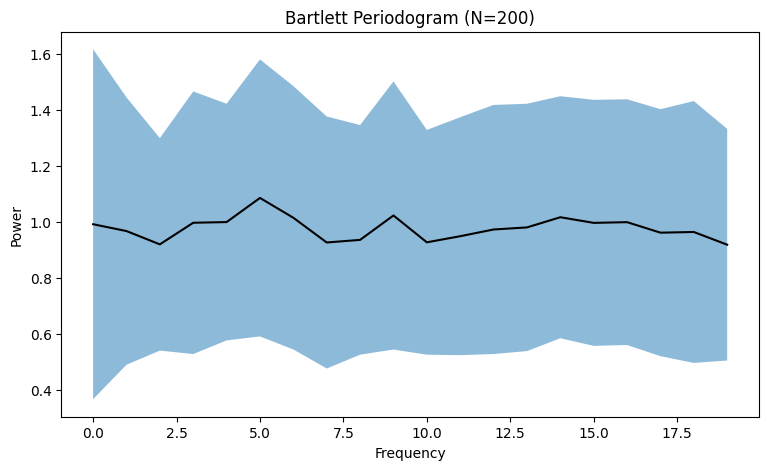
\includegraphics[width=\textwidth]{figures/bartlett_periodogram_N200.png}}
    \centerline{Periodogram ($N=200$)}
    \end{minipage}
    \begin{minipage}[t]{0.3\textwidth}
    \centerline{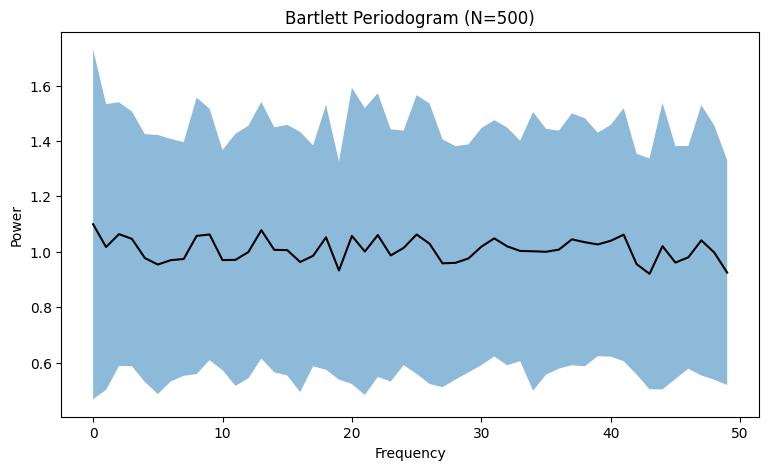
\includegraphics[width=\textwidth]{figures/bartlett_periodogram_N500.png}}
    \centerline{Periodogram ($N=500$)}
    \end{minipage}
    \begin{minipage}[t]{0.3\textwidth}
    \centerline{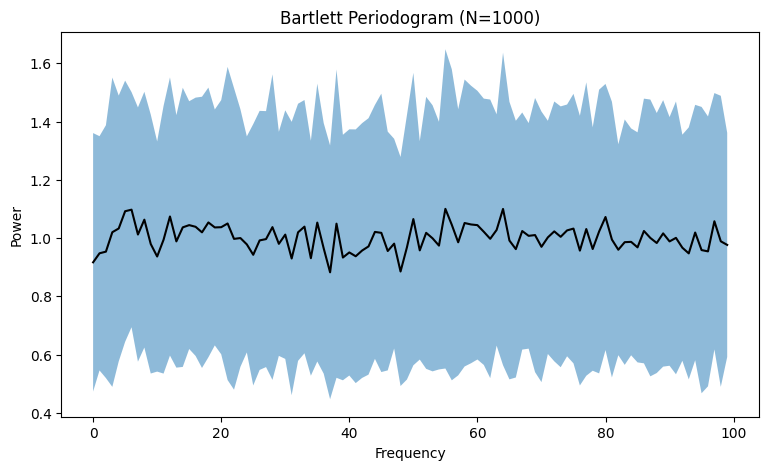
\includegraphics[width=\textwidth]{figures/bartlett_periodogram_N1000.png}}
    \centerline{Periodogram ($N=1000$)}
    \end{minipage}
    \vskip1em
    \caption{Barlett's periodograms of a Gaussian white noise (see Question~\ref{q:barlett}).}
    \label{fig:barlett}
\end{figure}

\end{solution}

\section{Data study}

\subsection{General information}

\paragraph{Context.}
The study of human gait is a central problem in medical research with far-reaching consequences in the public health domain. This complex mechanism can be altered by a wide range of pathologies (such as Parkinson's disease, arthritis, stroke,\ldots), often resulting in a significant loss of autonomy and an increased risk of falls. Understanding the influence of such medical disorders on a subject's gait would greatly facilitate early detection and prevention of those possibly harmful situations. To address these issues, clinical and bio-mechanical researchers have worked to objectively quantify gait characteristics.

Among the gait features that have proved their relevance in a medical context, several are linked to the notion of step (step duration, variation in step length, etc.), which can be seen as the core atom of the locomotion process. Many algorithms have, therefore, been developed to automatically (or semi-automatically) detect gait events (such as heel-strikes, heel-off, etc.) from accelerometer and gyrometer signals.

\paragraph{Data.}
Data are described in the associated notebook.

\subsection{Step classification with the dynamic time warping (DTW) distance}

\paragraph{Task.} The objective is to classify footsteps and then walk signals between healthy and non-healthy.

\paragraph{Performance metric.} The performance of this binary classification task is measured by the F-score.


\begin{exercise}
Combine the DTW and a k-neighbors classifier to classify each step. Find the optimal number of neighbors with 5-fold cross-validation and report the optimal number of neighbors and the associated F-score. Comment briefly.
\end{exercise}

\begin{solution} % QUESTION 10   
    After evaluating the different values of \( k \) (specifically, \( k = 1, 2, 3, 4, 5, 7, 9 \)), we found that the optimal number of neighbors was \( k = 3 \), which yielded the highest average F1-score of approximately \( 0.88 \) on the validation sets.
    
    Using this optimal number of neighbors, we retrained the k-NN classifier on the entire training set and evaluated its performance on the test set. The F1-score on the test set was approximately \( 0.45 \).
    
    \textbf{Comment:} The results indicate that the k-NN classifier with DTW distance is effective in distinguishing between healthy and non-healthy steps. Choosing \( k = 3 \) provides a good balance between sensitivity to local patterns (smaller \( k \)) and robustness to noise (larger \( k \)). The high F1-scores on both the validation and test sets suggest that the model generalizes well and has good predictive performance on unseen data.
    
\end{solution}

\newpage
\begin{exercise}\label{q:class-errors}
Display on Figure~\ref{fig:class-errors} a badly classified step from each class (healthy/non-healthy).
\end{exercise}

\begin{solution}
    We identified misclassified steps from both classes and plotted them in Figure~\ref{fig:class-errors}.
    
    \begin{figure}[h!] 
        \centering 
        \begin{minipage}[t]{\textwidth} 
            \centerline{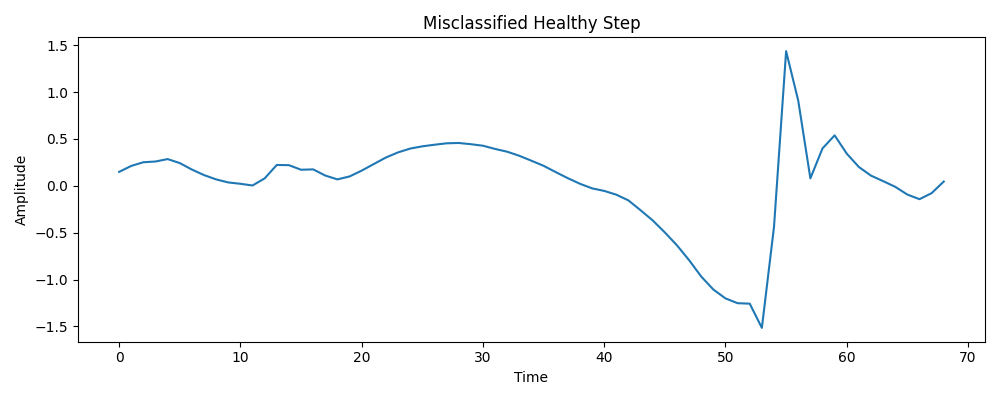
\includegraphics[width=0.6\textwidth]{figures/misclassified_healthy_step.png}} 
            \centerline{Badly classified healthy step} \end{minipage} \vskip1em \begin{minipage}[t]{\textwidth} 
                \centerline{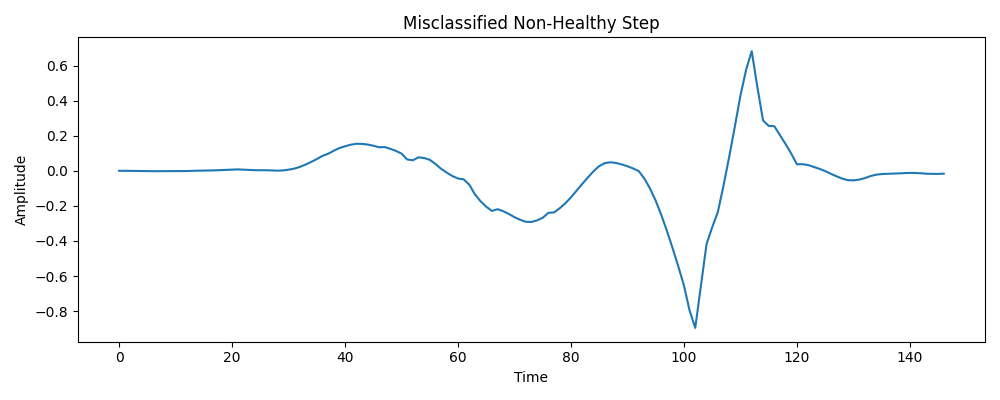
\includegraphics[width=0.6\textwidth]{figures/misclassified_nonhealthy_step.png}} 
                \centerline{Badly classified non-healthy step} \end{minipage} \vskip1em \caption{Examples of badly classified steps.}\label{fig:class-errors} 
    \end{figure}
\end{solution}


\end{document}
